\section{Kiến trúc tổng thể}

Việt Food áp dụng kiến trúc client-server hiện đại, với sự phân chia rõ ràng giữa frontend (React) và backend (Node.js/Express). Kiến trúc này tạo nên một hệ thống linh hoạt và mạnh mẽ, mang lại nhiều lợi ích:

\begin{itemize}
    \item \textbf{Phát triển độc lập}:
    \item \textbf{Khả năng mở rộng}
    \item \textbf{Tái sử dụng API}
    \item \textbf{Bảo mật tốt hơn}
    \item \textbf{Hiệu suất tối ưu}
\end{itemize}

\subsection{Mô hình kiến trúc}
Hệ thống áp dụng kiến trúc MVC (Model-View-Controller) kết hợp với các dịch vụ (Services):

\begin{itemize}
    \item \textbf{Model}: Đại diện cho cấu trúc dữ liệu và xử lý logic liên quan đến dữ liệu.
    \item \textbf{View}: Được thực hiện ở phía client, hiển thị thông tin cho người dùng.
    \item \textbf{Controller}: Xử lý các yêu cầu từ client, tương tác với các service và trả về kết quả.
    \item \textbf{Service}: Chứa logic nghiệp vụ, tương tác với database và các thành phần bên ngoài.
\end{itemize}

\subsection{Sơ đồ kiến trúc}
Kiến trúc hệ thống được thiết kế với nhiều lớp:
% add image here
\begin{figure}[H]
\centering  
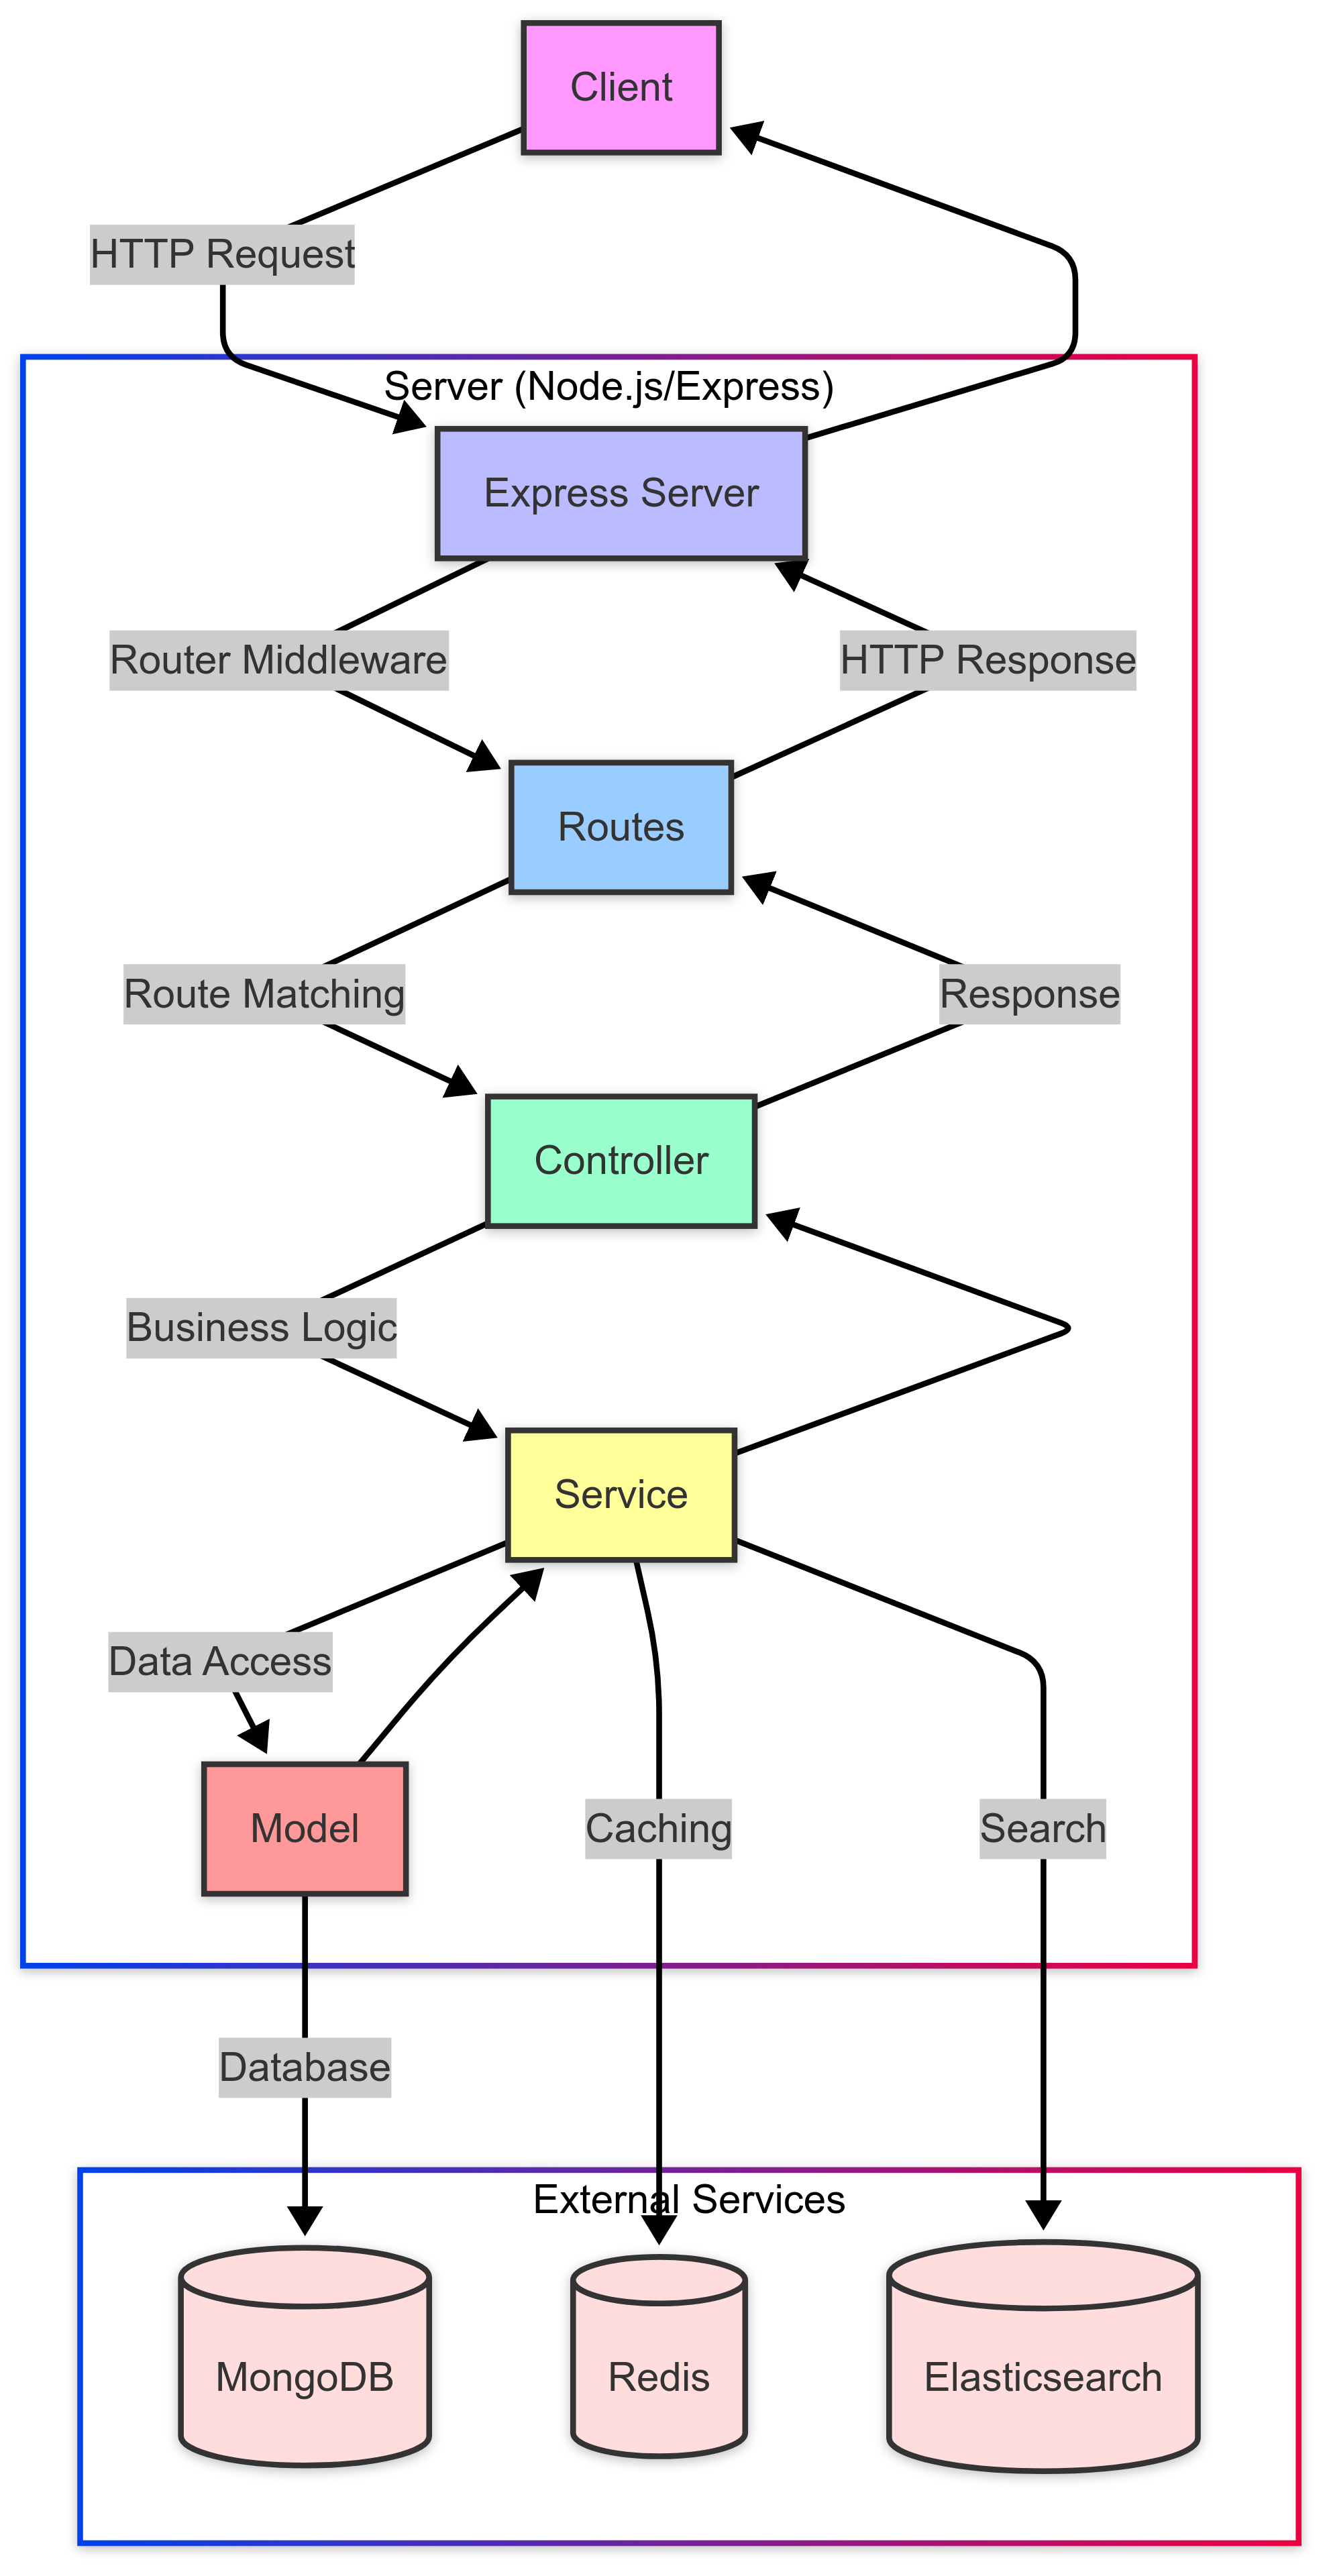
\includegraphics[width=0.8\textwidth]{images/architecture.png}
\caption{Sơ đồ kiến trúc tổng thể của hệ thống Việt Food}
\end{figure}


\section{Thiết kế module/component chính}
Cấu trúc dự án được tổ chức thành các module chức năng riêng biệt, gồm cả phần frontend và backend:

\subsection{Controllers}
Xử lý các request từ client và điều phối các thao tác:
\begin{itemize}
    \item \textbf{DishController}: Quản lý thông tin món ăn
    \item \textbf{CategoryController}: Quản lý danh mục
    \item \textbf{AuthController}: Xử lý xác thực người dùng
    \item \textbf{OrderController}: Xử lý đơn hàng
    \item \textbf{PaymentController}: Xử lý thanh toán
    \item \textbf{UserController}: Xử lý thông tin người dùng
    \item \textbf{UserProfileController}: Xử lý thông tin cá nhân
    \item \textbf{AgentController}: Xử lý tin nhắn chat
    \item \textbf{DashboardController}: Xử lý thống kê
\end{itemize}

\subsection{Services}
Chứa logic nghiệp vụ chính:
\begin{itemize}
    \item \textbf{DishService}: Xử lý logic liên quan đến món ăn, bao gồm caching với Redis
    \item \textbf{CategoryService}: Quản lý danh mục món ăn
    \item \textbf{AuthService}: Xử lý đăng nhập, đăng ký và xác thực
    \item \textbf{SearchService}: Tương tác với Elasticsearch để tìm kiếm
    \item \textbf{PaymentService}: Xử lý thanh toán
    \item \textbf{OrderService}: Xử lý đơn hàng
    \item \textbf{UserService}: Xử lý thông tin người dùng
    \item \textbf{AgentService}: Xử lý tin nhắn chat
    \item \textbf{DashboardService}: Xử lý thống kê
    \item \textbf{MessageWorkerService}: Xử lý tin nhắn với Redis Stream
    \item \textbf{MessageService}: Xử lý tin nhắn
\end{itemize}

\subsection{Middlewares}
Xử lý các tác vụ trung gian:
\begin{itemize}
    \item \textbf{Authentication}: Kiểm tra và xác thực người dùng
    \item \textbf{ImageProcessor}: Xử lý và tối ưu hóa hình ảnh với Sharp
\end{itemize}

\subsection{Models}
Mô tả cấu trúc dữ liệu chính trong backend:
\begin{itemize}
    \item \textbf{DishModel}: Mô hình dữ liệu cho món ăn
    \item \textbf{CategoryModel}: Mô hình dữ liệu cho danh mục
    \item \textbf{UserModel}: Mô hình dữ liệu người dùng
    \item \textbf{MessageModel}: Mô hình dữ liệu tin nhắn
    \item \textbf{OrderModel}: Mô hình dữ liệu đơn hàng
    \item \textbf{PaymentModel}: Mô hình dữ liệu thanh toán
\end{itemize}

\subsection{Frontend Components}
Frontend được xây dựng theo kiến trúc component-based với React, tổ chức thành các thành phần:
\begin{itemize}
    \item \textbf{UI Components}: Các component giao diện cơ bản, được xây dựng trên Radix UI và tùy chỉnh với Tailwind CSS
    \item \textbf{Layout Components}: Quản lý bố cục chung của ứng dụng
    \item \textbf{Page Components}: Tương ứng với các trang trong ứng dụng
\end{itemize}

\subsection{Frontend Services và Hooks}
Phần frontend sử dụng các service và custom hooks để quản lý logic:
\begin{itemize}
    \item \textbf{API Services}: Xử lý các tương tác với backend thông qua axios
    \item \textbf{Context API}: Sử dụng React Context để quản lý trạng thái toàn cục như xác thực người dùng (CartContext, AuthContext)
    \item \textbf{Custom Hooks}: Các hooks chuyên biệt như useAuth, useCart, useProfile để đơn giản hóa quản lý trạng thái và data fetching
    \item \textbf{Local Storage}: Lưu trữ tokens xác thực và thông tin session người dùng
\end{itemize}

\subsection{Quản lý Routing}
Việt Food sử dụng thư viện wouter để quản lý routing trong ứng dụng, với các route chính:
\begin{itemize}
    \item \textbf{Public Routes}: Trang chủ, danh sách món ăn, chi tiết món ăn, tìm kiếm
    \item \textbf{Protected Routes}: Giỏ hàng, quản lý đơn hàng, tài khoản cá nhân
    \item \textbf{Admin Routes}: Quản lý món ăn, danh mục, người dùng và thống kê
\end{itemize}

\subsection{State Management}
Quản lý trạng thái trong ứng dụng được thực hiện thông qua:
\begin{itemize}
    \item \textbf{React Context}: Quản lý trạng thái toàn cục như thông tin người dùng, giỏ hàng
    \item \textbf{Local Component State}: Quản lý trạng thái độc lập của từng component
\end{itemize}

\section{Thiết kế cơ sở dữ liệu}
Hệ thống sử dụng MongoDB làm cơ sở dữ liệu chính với thiết kế schema linh hoạt, phù hợp với đặc thù của ứng dụng đặt đồ ăn. Các collection chính được thiết kế như sau:

\subsection{Các collection chính}
\begin{itemize}
    \item \textbf{Users}: Quản lý thông tin người dùng
    \begin{itemize}
        \item \texttt{username}, \texttt{email}: Thông tin đăng nhập (duy nhất)
        \item \texttt{password}: Mật khẩu đã được mã hóa
        \item \texttt{role}: Phân quyền người dùng (USER/ADMIN)
        \item \texttt{isActive}: Trạng thái tài khoản
    \end{itemize}
    
    \item \textbf{Dishes}: Quản lý thông tin món ăn
    \begin{itemize}
        \item \texttt{name}, \texttt{description}: Thông tin cơ bản
        \item \texttt{price}, \texttt{imageUrl}: Giá và hình ảnh
        \item \texttt{category}: Tham chiếu đến danh mục
        \item \texttt{rating}, \texttt{soldCount}: Đánh giá và số lượng bán
        \item \texttt{isAvailable}, \texttt{isPopular}, \texttt{isNewDish}, \texttt{isSpecial}: Các cờ trạng thái
    \end{itemize}
    
    \item \textbf{Orders}: Quản lý đơn hàng
    \begin{itemize}
        \item \texttt{userId}: Người đặt hàng
        \item \texttt{orderItems}: Danh sách món đã đặt
        \item \texttt{totalAmount}: Tổng tiền
        \item \texttt{status}: Trạng thái đơn hàng
        \item \texttt{address}: Thông tin giao hàng
    \end{itemize}
    
    \item \textbf{Messages}: Lưu trữ lịch sử chat
    \begin{itemize}
        \item \texttt{userId}: Người gửi
        \item \texttt{content}: Nội dung tin nhắn
        \item \texttt{role}: Loại người gửi (user/assistant)
    \end{itemize}
\end{itemize}

\begin{figure}[H]
\centering  
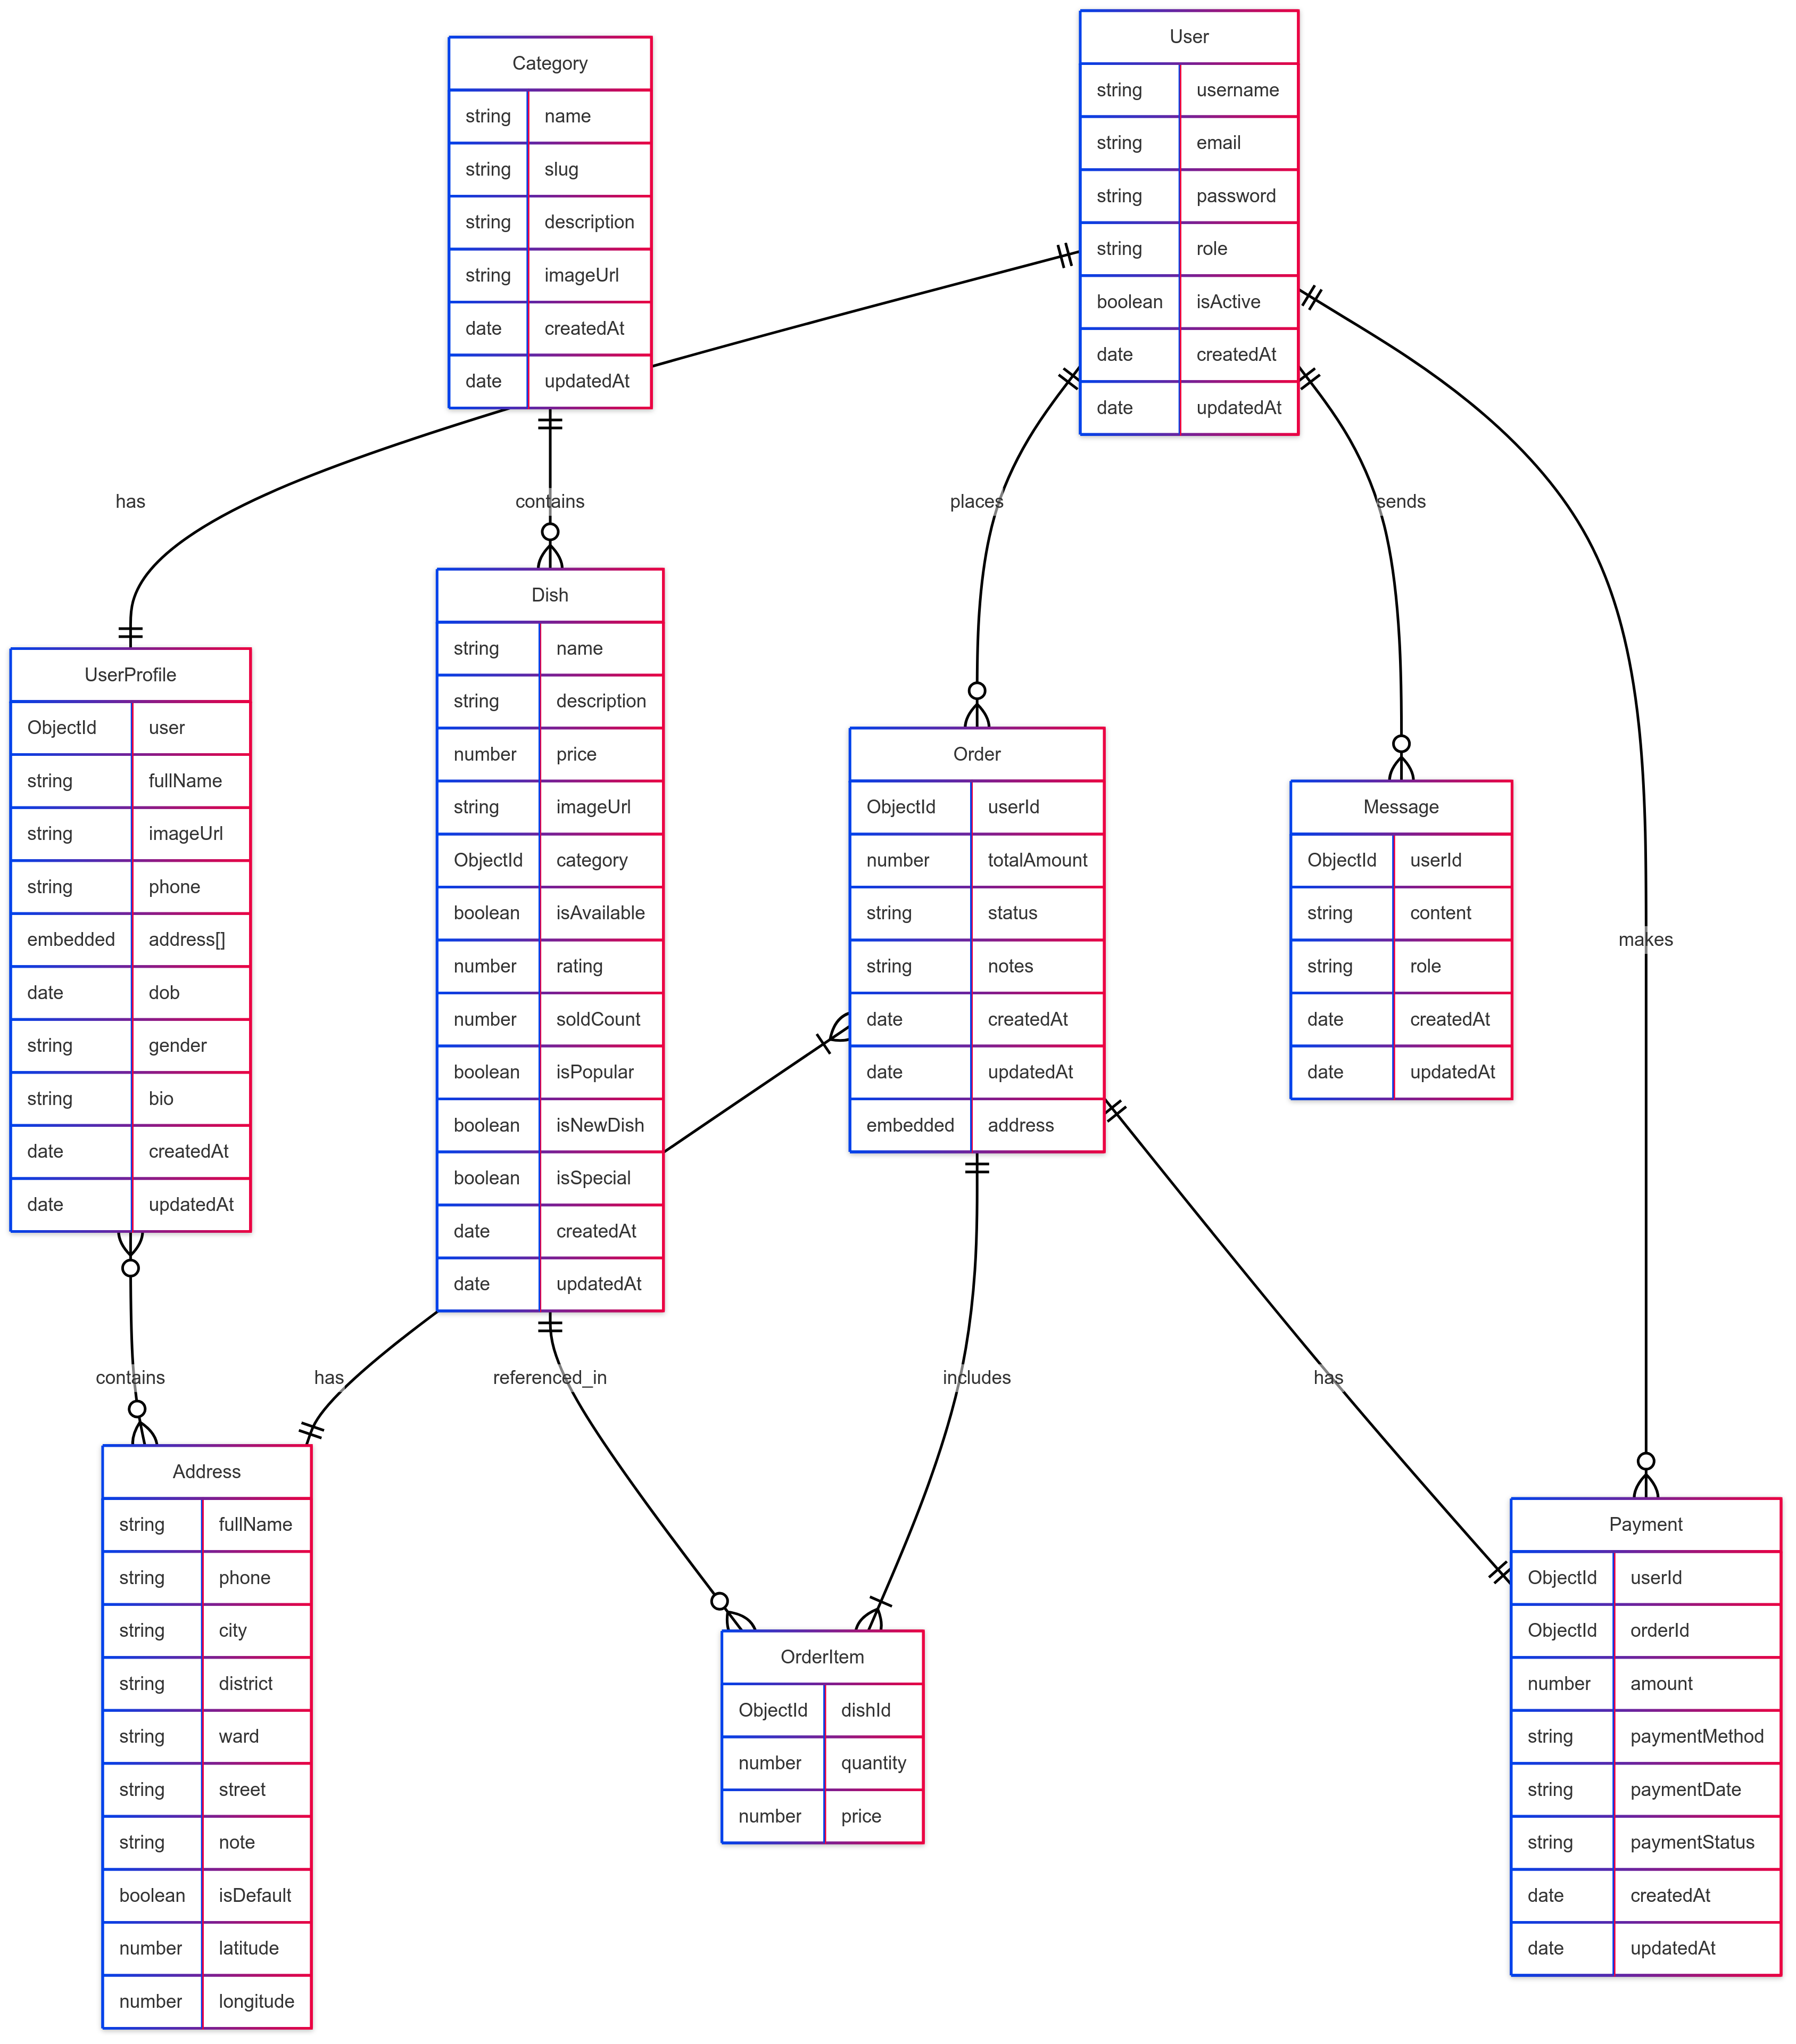
\includegraphics[width=\textwidth]{images/database-diagram.png}
\caption{Sơ đồ cơ sở dữ liệu của hệ thống Việt Food}
\label{fig:database-diagram}
\end{figure}

\subsection{Cơ sở dữ liệu bổ sung}
Bên cạnh MongoDB, hệ thống còn tích hợp:
\begin{itemize}
    \item \textbf{Redis}:
    \begin{itemize}
        \item Caching dữ liệu thường truy cập (thông tin món ăn, danh mục)
        \item Quản lý phiên đăng nhập
        \item Xử lý tin nhắn real-time thông qua Redis Stream
    \end{itemize}
    
    \item \textbf{Elasticsearch}:
    \begin{itemize}
        \item Đánh chỉ mục dữ liệu món ăn
        \item Hỗ trợ tìm kiếm full-text với khả năng ranking
        \item Tìm kiếm gợi ý (suggestions) khi người dùng nhập
    \end{itemize}
\end{itemize}

\subsection{Tối ưu hóa hiệu năng}
\begin{itemize}
    \item \textbf{Indexing}: Các trường thường xuyên truy vấn được đánh index
    \item \textbf{Caching}: Sử dụng Redis để giảm tải cho database chính
    \item \textbf{Phân trang}: Áp dụng cho danh sách món ăn và lịch sử đơn hàng
    \item \textbf{Aggregation}: Tổng hợp dữ liệu thống kê hiệu quả
\end{itemize}

\subsection{Bảo mật dữ liệu}
\begin{itemize}
    \item Mã hóa mật khẩu bằng bcrypt
    \item Xác thực JWT cho API
    \item Phân quyền chi tiết theo vai trò
    \item Kiểm tra quyền truy cập ở tầng middleware
\end{itemize}
